%\documentclass[a4paper, 12pt]{book}
\documentclass[oneside]{book}
%\usepackage[top=2cm, bottom=2cm, left=2.5cm, right=2.5cm]{geometry}
\usepackage[a4paper]{geometry}
\usepackage[utf8]{inputenc}
\usepackage[T1]{fontenc}
%\usepackage[portuguese]{babel}
\usepackage[brazil,english]{babel}
\usepackage{amsmath}
\usepackage{amsfonts}
\usepackage{amssymb}
\usepackage{mathtools}
\usepackage{listings}
\usepackage{xcolor}
\usepackage{verbatim}
\usepackage{graphicx}
\usepackage{enumerate} %listas numeradas
\usepackage{comment}
\usepackage{multicol}
\usepackage{minted}

% configurações
\lstset{
    language=C++,
	basicstyle=\normalsize\ttfamily,
	frame=single,
	tabsize=4,
	showstringspaces=false,
	commentstyle=\color{gray},
	keywordstyle=\color{blue},
	stringstyle=\color{orange},
}

\geometry{
	a4paper,
	left=10mm,
	right=10mm,
	top=1in,
	bottom=1in,
}

% tag Dedicatória
\newenvironment{dedication}
{
    \thispagestyle{empty}
    \vspace*{\stretch{20}}
    \itshape             
    \raggedleft
}{
    \par
    \vspace{\stretch{3}}
    \clearpage
}

\begin{document}

% Capa do Livro
\newcommand\nbvspace[1][3]{\vspace*{\stretch{#1}}}
\newcommand\nbstretchyspace{\spaceskip0.5em plus 0.25em minus 0.25em}
\newcommand{\nbtitlestretch}{\spaceskip0.6em}
\pagestyle{empty}
\begin{center}
	\bfseries
	\nbvspace[1]
	\Huge{\nbtitlestretch\huge BYTEMAIN'S ARSENAL}\\
	\nbvspace[1]
	\normalsize
	OS MELHORES ALGORITMOS REUNIDOS EM UM ÚNICO LIVRO.
	\nbvspace[1]\\
	\Large MAYCON D. A. SILVA\\[0.5em]
	\Large BRUNO R. LIMA\\[0.5em]
	\Large NATHAN A. SACRAMENTO\\[0.5em]
	\nbvspace[2]
	
\includegraphics[width=1.5in]{./config/Batman-logo.jpeg}\\
	\nbvspace[3]
	\normalsize
	\large
	PRIMEIRA EDIÇÃO
	\nbvspace[1]
\end{center}

% Dedicatórias
\begin{dedication}
\Large{Ao nosso técnico Ricardo Mesquita, por confiar em nós.}
\end{dedication}

% Sumário
\tableofcontents

% Vamos nos basear no contéudo do geeksforgeeks?
% Estou me baseando no cp-algorithms e codelibrary

\chapter{Táticas}
    \section{Limites de Representação de Dados}
        \begin{table}[h!]
\centering{
    \begin{tabular}{|c|c|c|ccc|c|}
    \hline
    tipo & scanf & bits & mínimo &..& máximo & precisão decimal\\
    \hline
    
    char & $\%c$ & $8$	& $0$ &..& $255$ & $2 $\\
    signed char & $\%hhd$ & $8 $& $-128$ &..& $127 	$ & $2 $\\
    unsigned char & $\%hhu$ & $8 $ & $0$ &..& $255 $ & $2 $\\
    short & $\%hd$ & $16$ & $-32.768$ &..& $32.767 $ & $4 $\\
    unsigned short & $\%hu$ & $16$ & $0$ &..& $65.535 $ & $4 $\\
    int & $\%d$ & $32$ 	& $-2 \times 10^9$ &..& $2 \times 10^9 $ & $9 $\\
    unsigned int & $\%u$ & $32$ & $0$ &..& $4 \times 10^9 $ & $9 $\\
    long long & $\%lld$ & $64$ & $-9 \times 10^{18}$ &..& $9 \times 10^{18} $ & $18$ \\
    unsigned long long & $\%llu$ & $64$ 	& $0$ &..& $18 \times 10^{18} 				$ & $19$ \\
    
    \hline
    \end{tabular}
}
\end{table}

\begin{table}[h!]
\centering{
    \begin{tabular}{|c|c|c|c|c|}
    \hline
    tipo & scanf & bits & expoente & precisão decimal \\
    \hline
    float & $\%f$ & 32 & 38 & 6 \\
    double & $\%lf$ & 64 & 308 & 15 \\
    long double & $\%Lf$ & 80 & 19.728 & 18 \\
    \hline
    \end{tabular}
}
\end{table}

\begin{table}[h!]
\centering{
    \begin{tabular}{|c|c|c|c|}
    \hline
    Fatorial & Valor & Fatorial & Valor\\
    \hline
    2! & 2 & 11! & 39.916.800\\
    3! & 6 & 12! & 479.001.600 (INT)\\
    4! & 24 & 13! & 6.227.020.800\\
    5! & 120 & 14! & 87.178.291.200\\
    6! & 720 & 15! & 1.307.674.368.000\\
    7! & 5.040 & 16! & 20.922.789.888.000\\
    8! & 40.320 & 17! & 355.687.428.096.000\\
    9! & 362.880 & 18! & 6.402.373.705.728.000\\
    10! & 3.682.800 & 19! & 121.645.100.408.832.000\\
    & & 20! & 2.432.902.008.176.640.000 (UNSIGNED LONG LONG)\\
    \hline
    \end{tabular}
}
\end{table}

\newpage

\section{Tabela ASCII}
\begin{figure}[h]
	\centering
	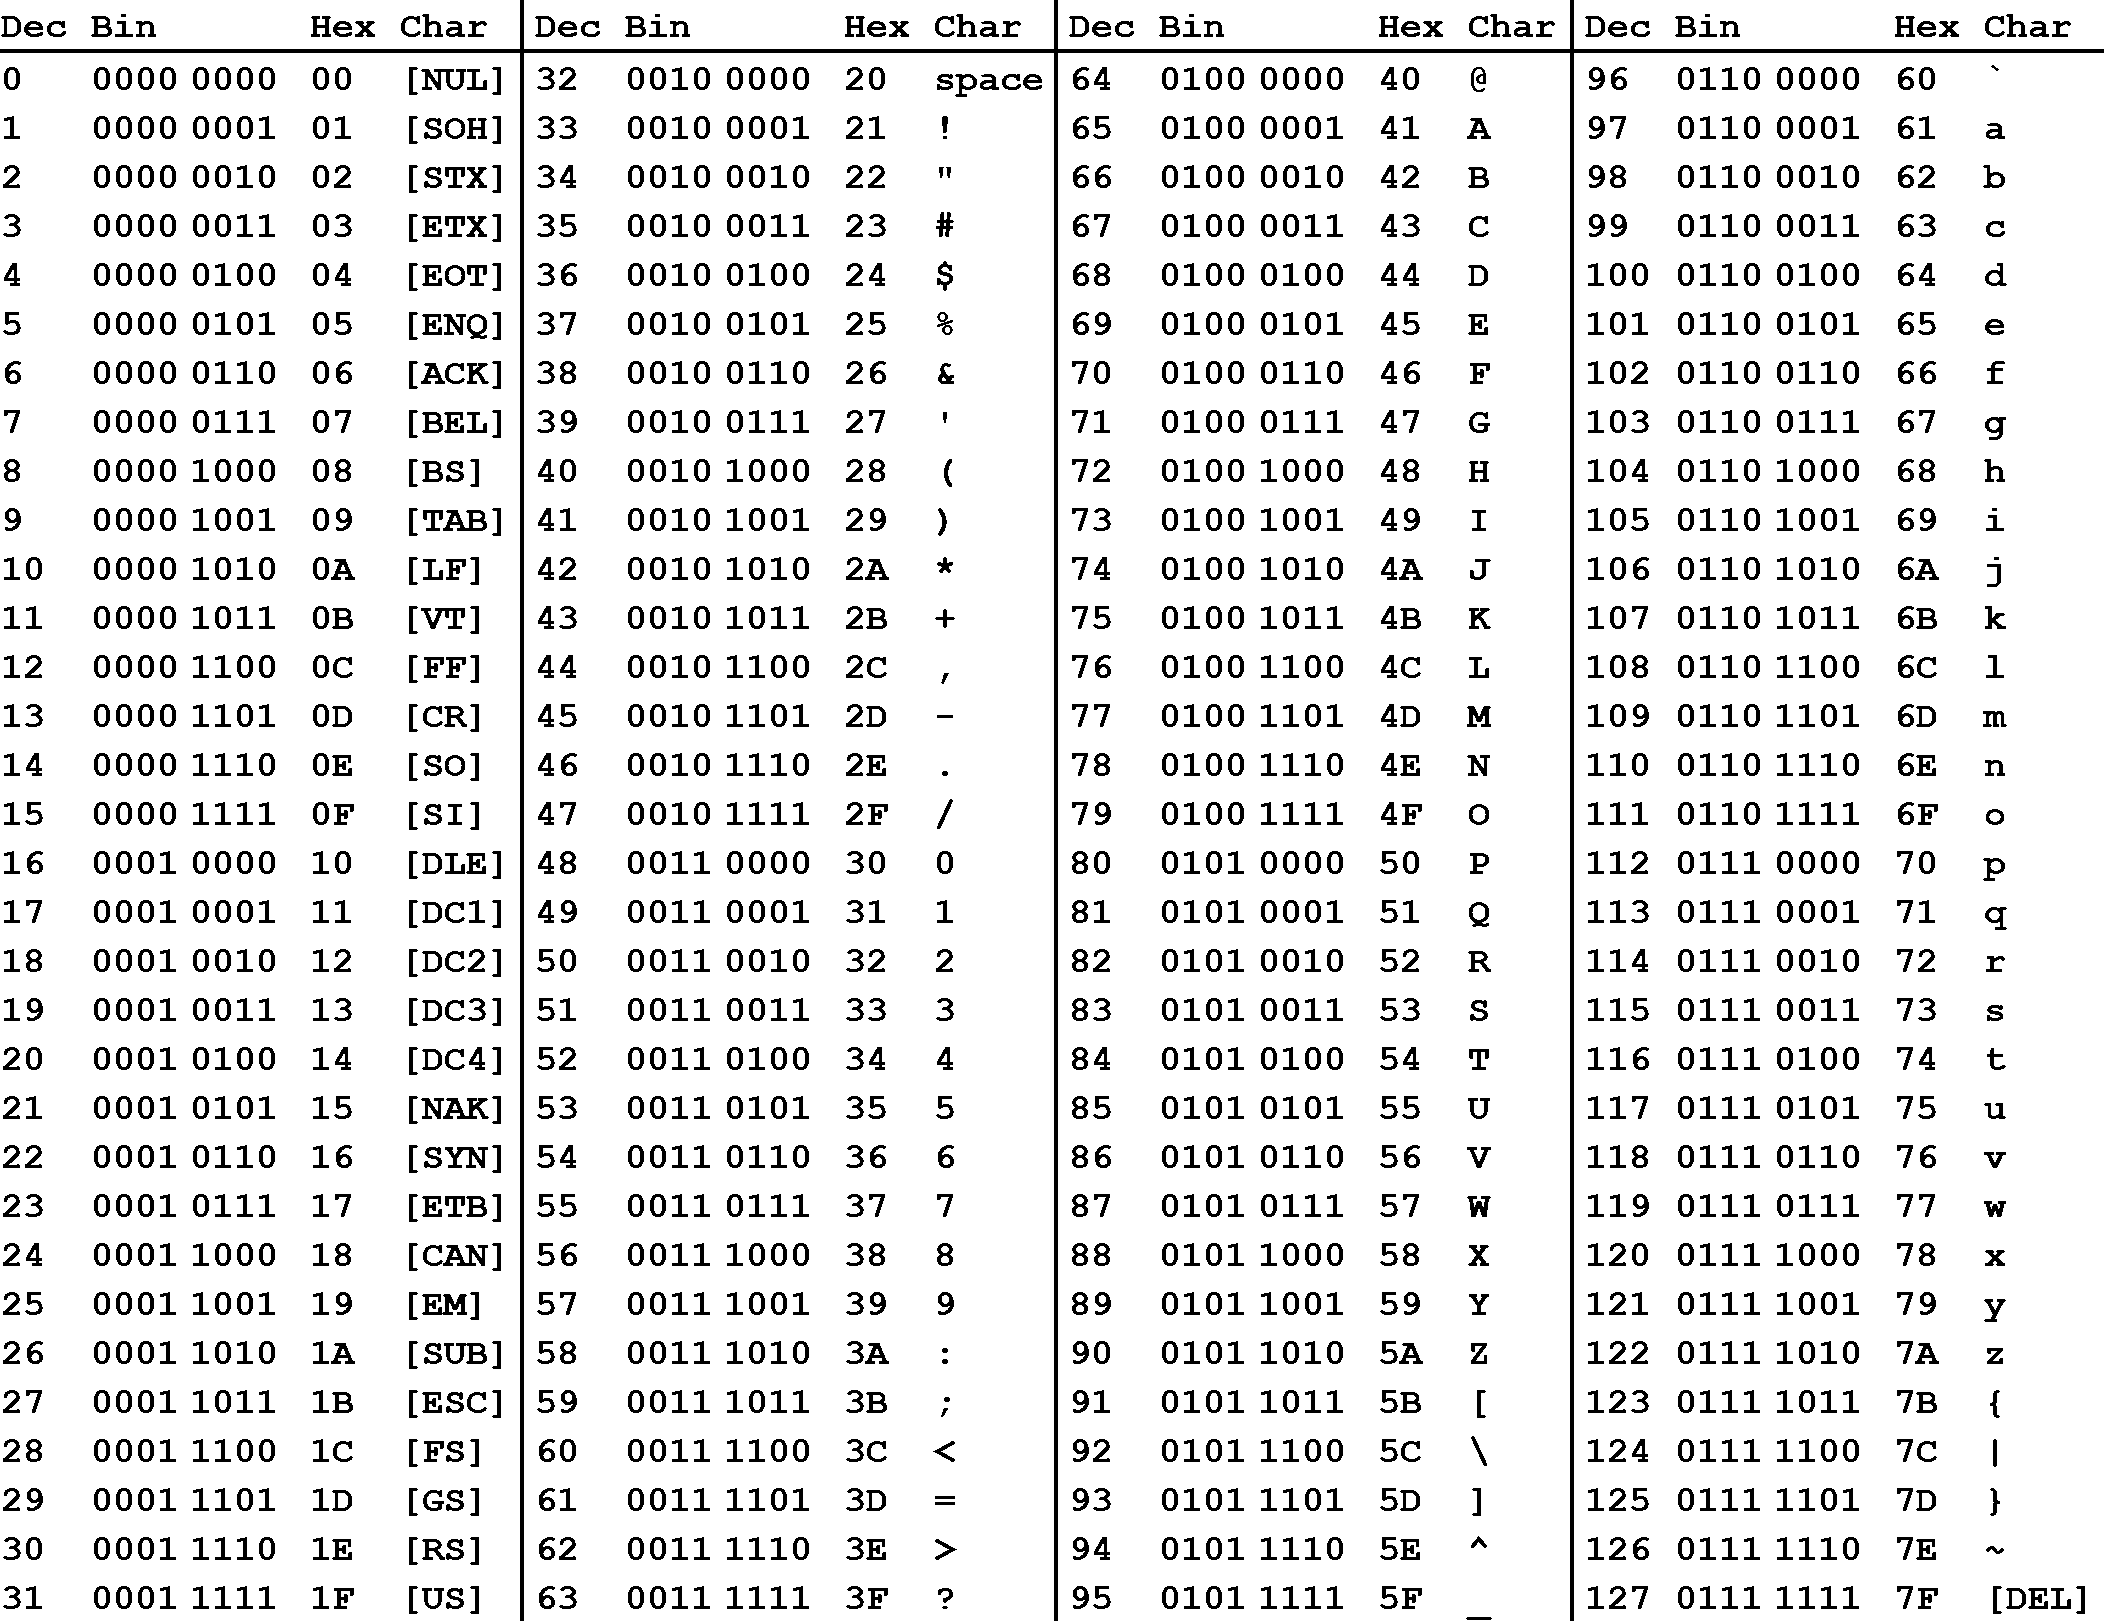
\includegraphics[width=\textwidth]{taticas/ascii.png}
\end{figure}

\newpage

\section{Tabela de Complexidades}
\begin{figure}[h]
	\centering
	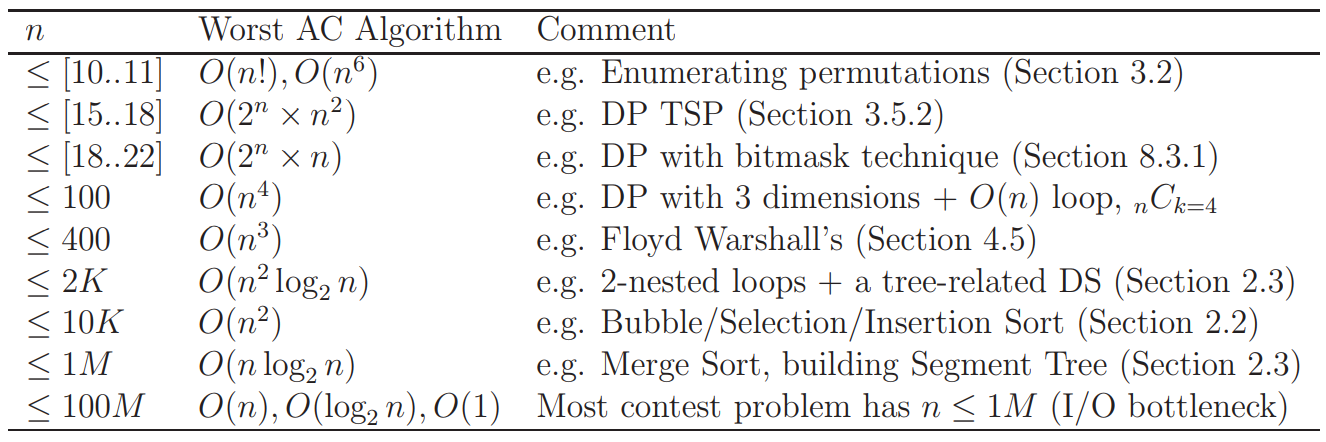
\includegraphics[width=\textwidth]{taticas/tab.png}
\end{figure}
        \newpage
    \section{Linguagens}
        \subsection*{C++}
\begin{lstlisting}[language=C++]
#define INF 0x3f3f3f3f
#define INFL 0x3f3f3f3f3f3f3f3f
#define b(x) bitset<x>
#define p(x) stack<x>
#define v(x) vector<x>
#define m(x) v(v(x))
#define d(x) deque<x>
#define l(x) list<x>
#define h(x, y) map<x, y>
#define s(x) set<x>
#define q(x) queue<x>
#define pq(x) priority_queue<x>
#define pub push_back
#define pob pop_back
#define puf push_front
#define pof pop_front
#define add insert
#define rm  erase
#define all(x) x.begin(), x.end()
#define par(x) pair<x, x>
\end{lstlisting}

\newpage

\subsection*{Python 3}
\begin{lstlisting}[language=Python, title={Tamanho da Pilha de Recursão}]
import sys
sys.setrecursionlimit(LIM)
\end{lstlisting}

\begin{lstlisting}[language=Python, title={Matriz}]
def matrix(linha,coluna,val):
	m = [None] * linha
	for i in range(0,linha):
		m[i] = [val] * coluna
	return m
\end{lstlisting}

\begin{lstlisting}[language=Python, title={Cortar Lista ou String }] 
sub_lista = lista[INICIO:FIM:SALTO]
\end{lstlisting}

\begin{lstlisting}[language=Python, title={Ler Até EOF}]
while True:
	try:
    	#codigo
    except EOFError:
    	break
\end{lstlisting}
\begin{lstlisting}[language=Python, title={Múltiplas Entradas na Mesma Linha}]
a, b, c = map(tipo, input().split("separador"))
\end{lstlisting}

\subsection*{Java}
\begin{lstlisting}[language=Java, title={Bibliotecas importantes}]
import java.math.BigInteger;
import java.util.*;
\end{lstlisting}

\begin{lstlisting}[language=Java, title={Conversão de Base}]
<TIPO>.toString(N, base);
\end{lstlisting}
        \newpage
    \section{Checklist}
        \chapter{Táticas de Ataque}
\section*{Pesquisa}
\begin{enumerate}
	\item{pesquisa linear}
	\item{primeiro, último, frequência, média, mediana, moda} 
	\item subsequência contínua de soma máxima
	\item necessidade de ordenar
	\item percursos em árvore: pre-ordem, em-ordem e pós-ordem
	\item Binary-Search
	\item jump-Search
	\item Indexação-Reversa
	\item map
	\item Segment tree
\end{enumerate}

\section*{Ordenação}
\section*{Grafos}
\section*{Bit}
\section*{Reconhecimento de Padrões}
\section*{Geometria Computacional}
\section*{Matemática}
        \newpage
    \section{Soluções de Problemas}
        \subsection*{Pesquisa}
Encontrar número que falta numa sequência?
Somar tudo e subtrair da soma gauss.\\
Caso a lista tenha saltos, deve fazer um FOR linear seguindo a regra de formação.

\subsection*{Mediana de duas Listas ordenadas}
Fazer um merge das duas listas,
calcular mediana normalmente.


        \newpage
\chapter{Matemática}
    \section{Combinatória}
        \subsection{Fórmulas}
            \begin{align*}
	\left(a+b\right)^{n} &= 
	\sum_{k=1}^{n} \binom{n}{k} a^{k} b^{n-k} & 
	\text{Catalan: } & 
	\frac{1}{n+1}\binom{2n}{n} &
	\text{Combinação com Repetição: } & 
	\binom{n-k-1}{k}
\end{align*}
        \subsection{Triângulo de Pascal}
            \begin{displaymath}
	\text{Regra de Formação: }
	\binom{n}{k}=\binom{n-1}{k-1}\binom{n-1}{k}\\\\
\end{displaymath}

\begin{lstlisting}[
    language=C++,
    emph={m, v, MAX_N, MAX_K}, emphstyle={\color{teal}}]
m(int) binomio(MAX_N + 1, v(int)(MAX_K + 1));
void generateBinomialTable() {
    for (int i = 0; i <= MAX_N; i++)
		for (int j = 0; j <= i; j++)
			binomio[i][j] = (j == 0) ? 1 :
            binomio[i-1][j-1] + binomio[i-1][j];
}
\end{lstlisting}
            \newpage
        \subsection{Troco Ótimo}
            \begin{lstlisting}[language = C++]
// n: total de moedas distintas, v: valor
int minCoins(V(int) coins, int n, int v) {
	V(int) dp(v + 1, INT_MAX); 
	dp[0] = 0;
    for (int i = 0; i < n; i++) dp[coins[i]] = 1;
    for (int i = 1; i <= v; i++)
    	for (int j = 0; j < n; j++)
        	if (i >= coins[j] and dp[i - coins[j]] != INT_MAX)
            	dp[i] = min(dp[i], dp[i - coins[j]] + 1);
    if (table[v] == INT_MAX) table[v] = -1;
    return table[v];
}
\end{lstlisting}
            \newpage
        \subsection{Mochila Bool}
            \begin{lstlisting}[language=c++, title=Itens acabam]
struct item { int v, p; }; // {valor, peso}
v(item) opcao;
m(int) memo;

int mochilaBool(int lim) { 
  const int n = opcao.size();
  // inicia tabela
  for(int i=0; i <n+1; i++) memo.pub(v(int)(lim+1,0));
  // bottom-up
  for(int i = 0; i <= n; i++){ 
    for(int j = 0; j <= lim; j++){ 
      if(i==0 or j==0) memo[i][j] = 0; 
      else if(opcao[i-1].p <= j) 
        // verifique a possibilidade de usar min();
        memo[i][j] = max(opcao[i-1].v
                     + memo[i-1][j-opcao[i-1].p], 
                     memo[i-1][j]); 
      else memo[i][j] = memo[i-1][j]; 
    } 
  } 
  return memo[n][lim]; 
}

// exe.: conteudoMochilaBool(LIM, mochilaBool(LIM));
void conteudoMochilaBool(int lim, int res){
  // desce a tabela 
  for(int i = opcao.size()-1; i > 0 && res > 0; i--){ 
    if( not(res == memo[i][lim])){ 
      printf("%d ", opcao[i].p); 
      res = res - opcao[i].v; 
      lim -= opcao[i].p; 
    } 
  } 
} 


\end{lstlisting}
        \subsection{Mochila Infinta}
            \begin{lstlisting}[language=c++, title=Itens nunca acabam]
struct item{ int v, p; };  
vector<item> opcao;
v(int) memo;

int mochilaInf(int lim) {
    const int n = opcao.size(); 
    // inicia tabela
    memo = v(int)(lim+1,0);
    // bottom-up
    for(int i=0; i<=lim; i++) 
        for(int j=0; j<n; j++) 
            if(opcao[j].p <= i) 
                memo[i] = max(memo[i], memo[i-opcao[j].p] 
                          + opcao[j].v); 
    return memo[lim]; 
}
\end{lstlisting}
            \newpage
        \subsection{Mochila Real}
            \begin{lstlisting}[language=c++, title=consegue quebrar os itens para caber]
struct item { int v, p; };
v(item) opcao;

double mochilaReal(int lim){
	const int n = opcao.size();
	int pesoAtual = 0; 
	double res = 0;

	sort(opcao.begin(), opcao.end(), 
	[](item &a, item &b)->bool{
		return (double)a.v / a.p > (double)b.v / b.p;
	});

	for (int i = 0; i < n; i++){
		if(pesoAtual + opcao[i].p <= lim){
			pesoAtual += opcao[i].p;
			res += opcao[i].v;
		}else{
			res += opcao[i].v * (double) (lim - pesoAtual) 
			       / opcao[i].p;
			break;
		}
	}

	return res;
}
\end{lstlisting}
        \subsection{Kadane, lista de Soma Máxima Contínua}
            \begin{lstlisting}[language = Python]
def kadane(lista):
	maximo = lista[0]
	maximo_aqui = lista[0] 
	for i in range(1,len(lista)):
		maximo_aqui = max(lista[i], maximo_aqui + lista[i])
		maximo = max(maximo, maximo_aqui)   
	return maximo
\end{lstlisting}
    \section{Recorrências}
        \subsubsection{Fibonacci (1, 1, 2, 3, 5, 8, 13, 21, 34, 55, 89, 144, 233, 377, 610, 987, 1597...)}
\begin{flalign*}
	f_{n} = \begin{cases}
	1, & \mbox{if } n\geq 2 \\
	f_{n-1}+f_{n-2}, & \mbox{otherwise} 
	\end{cases} & \Rightarrow
	round(f_{n-1} * \phi)\;|\;
	\frac{(1 + \sqrt{5})^{n} - (1 - \sqrt{5})^{n}}{2^{n}\sqrt{5}}\;|\;
	\left\lfloor\frac{\phi^{n}}{\sqrt{5}} + \frac{1}{2}\right\rfloor
\end{flalign*}

\subsubsection{Lucas (2, 1, 3, 4, 7, 11, 18, 29, 47, 76, 123, 199, 322, 521, 843, 1364, 2207,...)}
\begin{flalign*}
	L_{n} = \begin{cases}
	2, & \mbox{if } n=0 \\
	1, & \mbox{if } n=1 \\
	L_{n-1}+L_{n-2}, & \mbox{otherwise} 
	\end{cases} & \Rightarrow
	\left(\frac{1 + \sqrt{5}}{2}\right)^n + \left(\frac{1 - \sqrt{5}}{2}\right)^n
\end{flalign*}

\subsubsection{Josephus (P/ k Saltos)}
\begin{flalign*}
	J_{n, k} = \begin{cases}
	1, & \mbox{if } n=1 \\
	\left(k-1+f(n-1,\;k)\right)\mod(n + 1), & \mbox{otherwise} 
	\end{cases}
\end{flalign*}

\subsubsection{Catalan (1, 1, 2, 5, 14, 42, 132, 429, 1430, 4862, 16796, 58786, 208012,...)}
\begin{flalign*}
	C_{n}= \begin{cases} 1, & \mbox{if } n=0 \\
	\sum_{i=0}^{n} C_{i} C_{n-i}, & \mbox{otherwise}
	\end{cases} & \Rightarrow
	\frac{1}{n+1}\binom{2n}{n} \;|\;
	\prod_{k=2}^{n} \frac{n+k}{k}
\end{flalign*}

\subsubsection{Resolução de RL's de 2a Ordem}
\begin{itemize}
	\item $\text{Base cases } T_{0} \text{ and } T_{1} \text{ ; }T_{n}=K_{1}*T_{n-1}\;\pm\;K_{2}*T_{n-2}$
	\item $\text{Solve the equation }r^{2}-K_{1}r^{1}-K_{2}r^{0}=0$
	\item $\text{The solution has the form }\alpha_{1}*r_{1}^{n}+ \alpha_{2}*r_{2}^{n}\text{ for two roots}$
	\item $\text{The solution has the form }\alpha_{1}*r_{0}^{n}+ \alpha_{2}*n*r_{0}^{n}\text{ for one root}$
	\item $\text{Use the base cases to find alpha constants by linear system}$
\end{itemize}
        \newpage
    \section{Teoria dos Números}
        \subsection{Fórmulas Úteis}
            \subsubsection*{Função Totiente de Euler (\(\phi\)) \{1, 1, 2, 2, 4, 2, 6, 4, 6, 4, 10, 4, 12, 6, 8, ...\}}
\large{\(\phi(n) = n \prod_{p | n} \left(1 - 1/p\right)\) -> Calcula o número de inteiros positivos menores que n e que são relativamente primos (coprimos [mdc(x, y) = 1]) a n}
\begin{lstlisting}[language=C++]
big phi(big n) {// primes gerado por Crivo
	big i = 0, p = primes[i], answer = n;
	while (p * p <= n) {
		if (n % p == 0) answer -= answer / p;
		while (n % p == 0) n /= p;
		p = primes[++i];
	}
	if (n != 1) answer -= answer / n;
	return answer;
}

big phi_linear(big n) {
    big answer = n;
    for (big i = 2; i * i <= n; i++) {
        if (n % i == 0) {
            while (n % i == 0) n /= i;
            answer -= answer / i;
        }
    }
    if (n > 1) answer -= answer / n;
    return answer;
}

v(int) generatePhi(int limit) {
    v(int) answer(limit + 1);
    for (int i = 1; i <= limit; i++) answer[i] = i;
    for (int i = 1; i <= limit; i++) {
        for (int j = i + i; j <= limit; j += i)
            answer[j] -= answer[i];
    }
    return answer;
}
\end{lstlisting}

\subsubsection*{Equações Diofantinas}
\large{
    São equações no formato \(Ax + By = C\), onde A, B e C são constantes, x e y são as incógnitas e todos os valores são inteiros.\\
    Se C é divisivel por gdc(A, B), a equação tem solução.\\
    Se um par (x, y) é uma solução, então todos os pares \(\left(x+\frac{kB}{gcd(A, B)}, y-\frac{kA}{gcd(A, B)}\right)\) também serão.
}
            \newpage
        \subsection{Exponenciação Rápida}
            \begin{multicols}{2}
\begin{itemize}
	\item $\left(a + b\right) \;\%\; c = 
	      \left(\left(a \;\%\; c\right) + 
	      \left(b \;\%\; c\right)\right) \;\%\; c$
	\item $\left(a - b\right) \;\%\; c = 
	      \left(\left[\left(a \;\%\; c\right) -
	      \left(b \;\%\; c\right)\right] + c\right) \;\%\; c$
	\item $\left(a \times b\right) \;\%\; c = 
	      \left(\left(a \;\%\; c\right) \times
	      \left(b \;\%\; c\right)\right) \;\%\; c$
	
	\vfill
	
	\item $\left(a \div b\right) \;\%\; c = 
	      \left(\left(a \;\%\; c\right) \times
	      \left(b^{-1} \;\%\; c\right)\right) \;\%\; c$
	\item $a^{b} \;\%\; c = \left(a \;\%\; c\right)^{b} \;\%\; c$
\end{itemize}
\end{multicols}

\begin{lstlisting}[language=C++, title=Algoritmo de Exponenciação Modular]
int fastPower(int x, int n, int MOD) {
    int y = x, result = 1;
    while (n > 0) {
        if (n & 1) result = (result % MOD * y % MOD) % MOD;
        y = (y % MOD * y % MOD) % MOD;
        n >>= 1;
    }
    return result;
}
\end{lstlisting}

            \newpage
        \subsection{Números Primos}
            \subsubsection{Testes de Primalidade}
\begin{lstlisting}[language=C++]
bool is_prime(big n) {
    if (n < 0) return is_prime(n * (-1));
    for (big i = 2; i * i < n; i++)
        if (n % i == 0) return false;
    return true;
}

bool is_prime_fast(big n) {
    if (n < 0) n = n * (-1);
    if (n < 5 || n % 2 == 0 || n % 3 == 0)
        return (n == 2 || n == 3);
    big limit = sqrt(n) + 2;
    for (big p = 5; p < limit; p += 6) {
        if (p < n && n % p == 0) return false;
        if ((p + 2) < n && n % (p + 2) == 0) return false;
    }
    return true; }
\end{lstlisting}

\subsubsection{Crivo de Eratóstenes}
\begin{lstlisting}[language=C++]
big sieve_size; bs(MAX) isp; v(big) primes;
void sieve(big n) {
    sieve_size = n + 1; isp.set(); isp[0] = isp[1] = 0;
    for (big i = 2; i <= sieve_size; i++) {
        if (isp[i])
            for (big j = (i * i); j <= sieve_size; j += i)
            isp[j] = 0;
        primes.pb(i); } }

bool is_prime_sieve(big n) {
    if (n <= sieve_size) return isp[n];
    for (int i = 0; (i < primes.size()) && 
                    (primes[i] * primes[i] <= n); i++) {
        if (n % primes[i] == 0) return false; }
    return true; }
\end{lstlisting}

\newpage

\subsubsection{Crivo de Atkin}
\begin{lstlisting}[language=C++]
v(int) atkinSieve(int limit) {
    v(int) sieve;
    if (limit > 2) sieve.pb(2);
    if (limit > 3) sieve.pb(3);
    v(bool) is_prime(limit + 1, false);
    for (int x = 1; x * x < limit; x++) {
        for (int y = 1; y * y < limit; y++) {
            // Main part of Sieve of Atkin
            int n = (4 * x * x) + (y * y);
            if (n <= limit && (n % 12 == 1 || n % 12 == 5))
                is_prime[n] = (is_prime[n] ^ true);
            n = (3 * x * x) + (y * y);
            if (n <= limit && n % 12 == 7)
                is_prime[n] = (is_prime[n] ^ true);
            n = (3 * x * x) - (y * y);
            if (x > y && n <= limit && n % 12 == 11)
                is_prime[n] = (is_prime[n] ^ true);
        }
    }

    // Mark all multiples of squares as non-prime
    for (int r = 5; r * r < limit; r++) {
        if (is_prime[r])
            for (int i = r * r; i < limit; i += r * r)
                is_prime[i] = false;
    }

    for (int a = 5; a <= limit; a++)
        if (is_prime[a]) sieve.pb(a);
    
    return sieve;
}
\end{lstlisting}

\newpage

\subsubsection{Fatoração de Primos}
\begin{lstlisting}[language=C++]
v(int) primeFactors(big n) {// primes gerado por Crivo
    v(int) factors; big index = 0, pf = primes[index];
    while ((pf * pf) <= n) {
        while (n % pf == 0) { n /= pf; factors.pb(pf); }
        pf = primes[++index]; }
    if (n != 1) { factors.pb(n); } return factors;
}

big number_of_divisors(big n) {
	big i = 0, p = primes[i], answer = 1;
	while (p * p <= n) {
		big power = 0;
		while (n % p == 0) { n /= p; power++; }
		answer *= (power + 1); p = primes[++i];
	}
	if (n != 1) { answer *= 2; } return answer;
}

big numDiffPF[MAXN];// num de fatores primos distintos
void genDiffPF() {
	memset(numDiffPF, 0, sizeof(numDiffPF));
	for (int i = 2; i < MAXN; i++) {
		if (numDiffPF[i] == 0)
			for (int j = i; j < MAXN; j += i) numDiffPF[j]++;
	}
}
\end{lstlisting}
            \newpage
        \subsection{Torre de Hanói}
            \begin{lstlisting}[language=C++]
// 2^n - 1 = qtd de movimentos
void hanoi(int n, char orig, char dest, char aux){
    if(n == 1){
        cout << "Move disco 1 de " << orig;
        cout << " para " << dest << endl;
    }
    else{
        hanoi(n-1, orig, aux, dest);
        cout << "Move disco " << n << " de ";
        cout << orig << " para " << dest << endl;
        hanoi(n-1, aux, dest, orig);
    }
}
\end{lstlisting}
    \section{Estatística (em Python)}
        \begin{lstlisting}[language=python, otherkeywords={as}]
import statistics as s
s.mean(dados); s.harmonic_mean(dados)
s.median(dados); s.median_low(dados); s.median_high(dados)
s.median_grouped(data, interval=Number)
s.mode(data)
s.pvariance(data, mu=Number); s.variance(data, xbar=Number)
s.pstdev(data, mu=Number); s.stdev(data, xbar=Number)
\end{lstlisting}
        \newpage
    \section{Álgebra Linear}
        \subsection{Matrizes}
            \section{Matrizes}
\begin{lstlisting}[language=C++]
//#define MOD 1234567891
#define MOD 1000000007
M(int) matrixUnit(int n) {
    M(int) res(n, V(int)(n));
    for (int i = 0; i < n; i++) res[i][i] = 1;
    return res;
}

M(int) matrixAdd(const M(int) &a, const M(int) &b) {
    int n = a.size();
    int m = a[0].size();
    M(int) res(n, V(int)(m));
    for (int i = 0; i < n; i++)
        for (int j = 0; j < m; j++)
            res[i][j] = (a[i][j] + b[i][j]) % MOD;
    return res;
}

M(int) matrixMul(const M(int) &a, const M(int) &b) {
    int n = a.size();
    int m = a[0].size();
    int k = b[0].size();
    M(int) res(n, V(int)(k));
    for (int i = 0; i < n; i++)
        for (int j = 0; j < k; j++)
            for (int p = 0; p < m; p++)
                res[i][j] = (res[i][j] + (big)
                			(a[i][p] * b[p][j]) % MOD) % MOD;
    return res;
}

M(int) matrixPow(const M(int) &a, int p) {
    if (p == 0) return matrixUnit(a.size());
    if (p & 1) return matrixMul(a, matrixPow(a, p - 1));
    return matrixPow(matrixMul(a, a), p / 2);
}

M(int) matrixPowSum(const M(int) &a, int p) {
    int n = a.size();
    if (p == 0) return M(int)(n, V(int)(n));
    if (p % 2 == 0)
        return matrixMul(matrixPowSum(a, p / 2),
        				 matrixAdd(matrixUnit(n), 
                        		   matrixPow(a, p / 2)));
    return matrixAdd(a, matrixMul(matrixPowSum(a, p - 1), a));
}
\end{lstlisting}
            \newpage
        \subsection{Determinantes}
            \input{matematica/algebra_linear/determinantes}
            \newpage
        \subsection{Sistemas Lineares}
            \subsubsection{Número de Soluções de uma Equação Linear}
\begin{lstlisting}[language=C++]
// a: coeficientes, b: resultado
int countSolutions(v(int) a, int b) {
    int dp[b + 1]; dp[0] = 1;
    for (int i = 0; i < a.size(); i++)
        for (int j = a[i]; j <= b; j++) dp[j] += dp[j-a[i]];
    return dp[b];
}
\end{lstlisting}
            \newpage
    \section{Matrix Chain Multiplication}
        \large{
    Dada uma sequência de matrizes, informe o número ótimo de multiplicações, ou seja, considerando que a operação de multiplicação de matrizes é associativa (ex: A(BC) <=> (AB)C), qual é a melhor maneira de multiplicar as matrizes, de modo a minimizar a quantidade de operações?\\
    Ex: A[10][30], B[30][5], C[5][60]\\
        (AB)C = (10*30*5) + (10*5*60) = 4500\\
        A(BC) = (30*5*60) + (10*30*60) = 27000
}
\begin{lstlisting}[language=C++]
int matrixChainMultiplication(v(int) matrix) {
    int n = matrix.size();
    int minimumCost[n][n];
    for (int i = 1; i < n; i++) minimumCost[i][i] = 0;
    for (int l = 2; l < n; l++) {
        for (int i = 1; i <= n - l; i++) {
            int j = i + l - 1;
            minimumCost[i][j] = INT_MAX;
            for (int k = i; k < j; k++) {
                int current = minimumCost[i][k] + 
                              minimumCost[k + 1][j] + 
                              matrix[i - 1] * matrix[k] * 
                              matrix[j];
                minimumCost[i][j] = min(minimumCost[i][j],
                                        current);
            }
        }
    }
    return minimumCost[1][n - 1];
}
\end{lstlisting}
        \newpage
    \section{Geometria Computacional}
        \subsection{Fórmulas}
            \begin{lstlisting}[language=C++]
#define EPS 1e-9
#define PI 3.14159265359
struct linha { double a, b, c; };
struct ponto {
	double x, y;
    bool operator<(const ponto &p) const {// util p/ sorting
    	if (fabs(this.x - p.x) > EPS) return this.x < p.x;
        return this.y < p.y;
    }
    bool operator==(const ponto &p) const {
    	return fabs(x - p.x) < EPS && fabs(y - p.y) < EPS;
    }
};
typedef struct { ponto centro; double raio; } circulo;

double distancia(Ponto p1, Ponto p2){ //distancia euclidiana
	return sqrt(pow((p1.x - p2.x), 2) + 
    			pow((p1.y - p2.y), 2));
}

ponto rotate(ponto p, double rad){
	return ponto(p.x * cos(rad) - p.y * sin(rad),
    			p.x * sin(rad) + p.y * sin(rad));
}

float area_tr_eq(float side){return sqrt(3)/4 * side * side;}
float peri_tr_eq(float side) { return 3 * side; }
float area_circunscrita(float a) {
    return (a * a * (PI / 3));
}

int rectCount(int n, int m){ //quantos retangulos num grid
    return (m * n * (n + 1) * (m + 1)) / 4;
}
\end{lstlisting}
            \newpage
        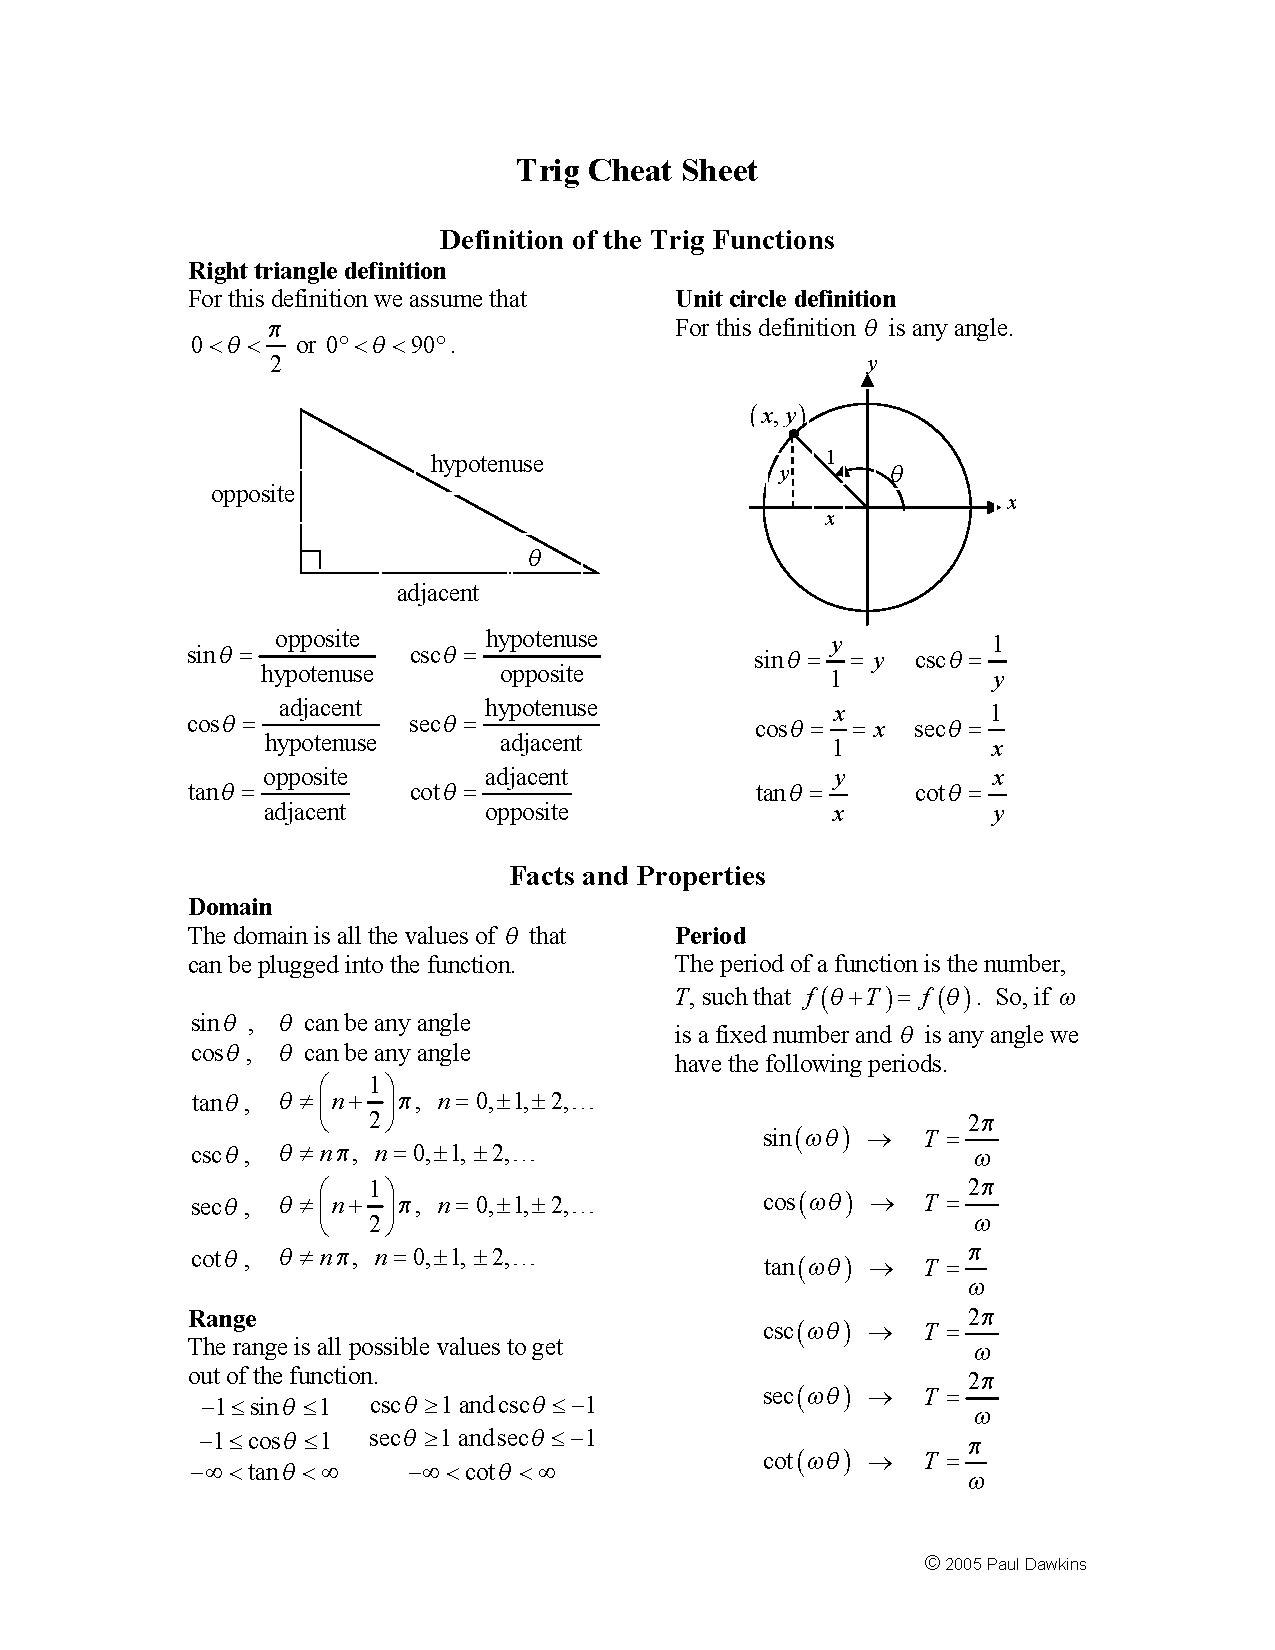
\includepdf[pages=1, pagecommand=\subsection{Trigonometria}]{matematica/geometria/trigonometry}
\newpage
\includepdf[pages=2-]{matematica/geometria/trigonometry}
        \subsection{Ponto}
            A implementação do ponto como struct ajuda a otimizar algumas operações - por conta da sobrecarga dos operadores, mas perde-se mais tempo escrevendo. Sempre que possível, dar preferência para $par(double)$ e adaptar as funções de ponto para tal tipo - o que é bastante rápido. Operações com Vetores utilizam as funções de ponto.

\begin{lstlisting}[language=C++, title=Parte 1: Estrutura]
struct point {
    double x, y; point(): x(0), y(0) {}
    point(double _x, double _y): x(_x), y(_y) {}
    
    double norm() { return hypot(x, y); }
    
    point normalized() {
        return point(x, y) * (1.0 / norm()); }
        
    double polarAngle() {
		double a = atan2(y, x);
		return a < 0 ? a + 2 * acos(-1.0) : a; }
		
	bool operator<(point other) const {
		if (fabs(x - other.x) > EPS) return x < other.x;
		else return y < other.y; }
    
	bool operator==(point other) const {
		return (fabs(x - other.x) < EPS && 
		       (fabs(y - other.y) < EPS)); }
    
	point operator+(point other) const {
		return point(x + other.x, y + other.y); }
    
	point operator-(point other) const {
		return point(x - other.x, y - other.y); }
		
	point operator*(double k) const {
		return point(x * k, y * k); }
};
\end{lstlisting}

\newpage

\begin{lstlisting}[language=C++, title=Parte 2: Operações]
double distance(point p1, point p2) {
	return hypot(p1.x - p2.x, p1.y - p2.y); }

double innerProduct(point p1, point p2) {
	return p1.x * p2.x + p1.y * p2.y; }

double crossProduct(point p1, point p2) {
	return p1.x * p2.y - p1.y * p2.x; }

bool ccw(point p, point q, point r) {
	return crossProduct(q - p, r - p) > 0; }

bool collinear(point p, point q, point r) {
	return fabs(crossProduct(p - q, r - p)) < EPS; }

point rotate(point p, double rad) {
	return point(p.x * cos(rad) - p.y * sin(rad), 
	             p.x * sin(rad) + p.y * cos(rad)); }

double angle(point a, point o, point b) {
	return acos(innerProduct(a - o, b - o) / 
	           (distance(o, a) * distance(o, b))); }

point proj(point u, point v) {
	return v * (innerProduct(u, v) / innerProduct(v, v)); }

bool between(point p, point q, point r) {
	return collinear(p, q, r) && inner(p - q, r - q) <= 0; }

point lineIntersectSeg(point p, point q, point A, point B) {
	double c = crossProduct(A - B, p - q);
	double a = crossProduct(A, B), b = crossProduct(p, q);
	return ((p - q) * (a / c)) - ((A - B) * (b / c)); }

bool parallel(point a, point b) {
	return fabs(crossProduct(a, b)) < EPS; }

\end{lstlisting}

\newpage

\begin{lstlisting}[language=C++, title=Parte 2: Operações (cont.)]
bool segIntersects(point a, point b, point p, point q) {
	if (parallel(a - b, p - q)) {
		return between(a, p, b) || between(a, q, b) || 
               between(p, a, q) || between(p, b, q); 
	}
	point i = lineIntersectSeg(a, b, p, q);
	return between(a, i, b) && between(p, i, q);
}

point closestToLineSegment(point p, point a, point b) {
	double u = inner(p - a, b - a) / inner(b - a, b - a);
	if (u < 0.0) return a; if (u > 1.0) return b;
	return a + ((b - a) * u); }

// Outra forma de saber o ccw
int ccw2(ponto &P0, ponto &P1, ponto &P2) {
    int dx1 = P1.x - P0.x, dx2 = P2.x - P0.x;
    int dy1 = P1.y - P0.y, dy2 = P1.y - P0.y;
    if (dy1 * dx2 > dy2 * dx1) return -1;
    if (dx1 * dy2 > dy1 * dx2) return 1;
    if ((dx1 * dx2 < 0) || (dy1 * dy2 < 0)) return 1;
    if ((dx1 * dx1 + dy1 * dy1) < (dx2 * dx2 + dy2 * dy2))
        return -1;
    return 0; }

// corssProduct p/ 3 pontos
int crossProduct2(ponto &O, ponto &A, ponto &B) {
	return (A.x - O.x) * (B.y - O.y) - 
	       (A.y - O.y) * (B.x - O.x); }

// usado p/ convexHull
bool angleCmp(point a, point b) {
	if (collinear(pivot, a, b))
		return inner(pivot - a, pivot - a) <
		       inner(pivot - b, pivot - b);
	return cross(a - pivot, b - pivot) >= 0;
}
\end{lstlisting}
            \newpage
        \subsection{Linha}
            \begin{lstlisting}[language=C++, title=Parte I de II]
struct line {
	double a, b, c;
	line() { a = b = c = NAN;}
	line(double a, double b, double c): a(a), b(b), c(c) {}
};

line pointsToLine(point p, point q) {
	if (fabs(p.x - q.x) < EPS && fabs(p.y - q.y) < EPS)
		return line();
	if (fabs(p.x - q.x) < EPS)
		return line(1.0, 0.0, -q.x);
	line l;
	l.a = -(p.y - q.y) / (p.x - q.x);
	l.b = 1.0;
	l.c = -(l.a * p.x) - p.y;
	return l;
}

bool areParallel(line l1, line l2) {
	return (fabs(l1.a - l2.a) < EPS) && 
	       (fabs(l1.b - l2.b) < EPS);
}

bool areSame(line l1, line l2) {
	return areParallel(l1, l2) && (fabs(l1.c - l2.c) < EPS);
}

point intersection(line l1, line l2) {
	if (areParallel(l1, l2)) return point(NAN, NAN);
	point p;
	p.x = (l2.b * l1.c - l1.b * l2.c) / 
	      (l2.a * l1.b - l1.a * l2.b);
	if (fabs(l1.b) > EPS) p.y = -(l1.a * p.x + l1.c);
	else p.y = -(l2.a * p.x + l2.c);
	return p;
}
\end{lstlisting}

\newpage

\begin{lstlisting}[language=C++, title=Parte II de II]
point projPointToLine(point u, line l) {
	point a, b;
	if (fabs(l.b - 1.0) < EPS) {
		a = point(-l.c / l.a, 0.0);
		b = point(-l.c / l.a, 1.0);
	} else {
		a = point(0, -l.c / l.b);
		b = point(1, -(l.c + 1.0) / l.b);
	}
	return a + proj(u - a, b - a);
}

double distToLine(point p, line l) {
	return dist(p, projPointToLine(p, l));
}
\end{lstlisting}
            \newpage
        \subsection{Circunferência}
            \begin{lstlisting}[language=C++, title=Parte I de II]
struct circle {
	point p; double raio;
	circle() { p = point(); raio = 0; }
	circle(point p, double raio): p(p), raio(raio) {}
	
	double area() { return acos(-1.0) * raio * raio; }
	
	double chord(double rad) {
	    return 2 * raio * sin(rad / 2.0); }
	    
	double sector(double rad) {
	    return 0.5 * rad * area() / acos(-1.0); }
	    
	bool intersects(circle other) {
		return dist(p, other.p) < raio + other.raio; }
		
	bool contains(point p) {
		return dist(this->p, p) <= raio + EPS; }
		
	// se o ponto estiver dentro asin retorna NAN
	pair<point, point> getTangentPoint(point p) {
		double d1 = dist(p, this->p);
		double theta = asin(raio / d1);
		point p1 = rotate(this->p - p, -theta);
		point p2 = rotate(this->p - p, theta);
		p1 = p1 * (sqrt(d1 * d1 - raio * raio) / d1) + p;
		p2 = p2 * (sqrt(d1 * d1 - raio * raio) / d1) + p;
		return make_pair(p1, p2);
	}
};
\end{lstlisting}

\newpage

\begin{lstlisting}[language=C++, title=Parte II de II]
circle circumcircle(point a, point b, point c) {
	circle answer;
	point u = point((b - a).y, -(b - a).x);
	point v = point((c - a).y, -(c - a).x);
	point n = (c - b) * 0.5;
	double t = crossProduct(u, n) / crossProduct(v, u);
	answer.p = ((a + c) * 0.5) + (v * t);
	answer.raio = dist(answer.p, a);
	return answer;
}

int insideCircle(point p, circle c) {
	if (fabs(dist(p , c.p) - c.raio) < EPS) return 1;//border
	if (dist(p , c.p) < c.raio) return 0;//inside
	return 2;//outside
}

// divisao por zero se os pontos forem colineares
circle incircle(point p1, point p2, point p3) {
    double m1 = dist(p2, p3);
    double m2 = dist(p1, p3);
    double m3 = dist(p1, p2);
    point c = (p1 * m1 + p2 * m2 + p3 * m3) * 
              (1 / (m1 + m2 + m3));
    double s = 0.5 * (m1 + m2 + m3);
    double r = sqrt(s * (s - m1) * (s - m2) * (s - m3)) / s;
    return circle(c, r);
}
\end{lstlisting}
            \newpage
        \subsection{Triângulo}
            \subsubsection*{Tipos de Triângulo}
\begin{itemize}
\item Equilátero: todos os lados são iguais
\item Isósceles: dois lados e dois ângulos iguais
\item Escaleno: não tem dois lados e dois ângulos iguais
\item Retângulo: tem um ângulo reto
\item Obtusângulo:  tem um ângulo obtuso, ou seja, maior que 90 graus
\item Acutângulo: todos os seus ângulos são agudos, ou seja, menores que 90 graus
\end{itemize}

\subsubsection*{Condições para a Existência de um Triângulo}
\centering{
\(1.\;| b - c | < a < b + c\;\;\;\)
\(2.\;| a - c | < b < a + c\;\;\;\) 
\(3.\;| a - b | < c < a + b\)
}
            \newpage
        \subsection{Polígono}
            \begin{lstlisting}[language=C++, title=Parte I de II]
typedef vector<point> polygon;

double signedArea(polygon &P) {
	double result = 0.0; int n = P.size();
	for (int i = 0; i < n; i++)
		result += crossProduct(P[i], P[(i + 1) % n]);
	return result / 2.0;
}

int leftMostIndex(polygon &P) {
	int answer = 0;
	for(int i = 1; i < (int) P.size(); i++)
		if (P[i] < P[answer]) answer = i;
	return answer;
}

polygon makePolygon(vector<point> P) {
	if (signedArea(P) < 0.0) reverse(P.begin(), P.end());
	int li = leftMostIndex(P);
	rotate(P.begin(), P.begin() + li, P.end());
	return P;
}

double perimeter(polygon &P) {
	double result = 0.0;
	int n = (int) P.size();
	for (int i = 0; i < n; i++)
		result += dist(P[i], P[(i + 1) % n]);
	return result;
}

double area(polygon &P) {
	return fabs(signedArea(P));
}
\end{lstlisting}

\newpage

\begin{lstlisting}[language=C++, title=Parte II de II]
bool isConvex(polygon &P) {
	int n = P.size();
	if (n < 3) return false;
	bool left = ccw(P[0], P[1], P[2]);
	for (int i = 1; i < n; i++)
		if (ccw(P[i], P[(i + 1) % n], 
		        P[(i + 2) % n]) != left)
			return false;
	return true;
}

bool inPolygon(polygon &P, point p) {
	if ((int) P.size() == 0) return false;
	double sum = 0.0; int n = P.size();
	for (int i = 0; i < n; i++) {
		if (P[i] == p || between(P[i], p, P[(i + 1) % n]))
			return true;
		if (ccw(p, P[i], P[(i + 1) % n]))
			sum += angle(P[i], p, P[(i + 1) % n]);
		else
			sum -= angle(P[i], p, P[(i + 1) % n]);
	}
	return fabs(fabs(sum) - 2 * acos(-1.0)) < EPS;
}

polygon cutPolygon(polygon &P, point a, point b) {
	vector<point> R; double left1, left2; int n = P.size();
	for (int i = 0; i < n; i++) {
		left1 = crossProduct(b - a, P[i] - a);
		left2 = crossProduct(b - a, P[(i + 1) % n] - a);
		if (left1 > -EPS) R.push_back(P[i]);
		if (left1 * left2 < -EPS)
			R.push_back(lineIntersectSeg(
			            P[i], P[(i + 1) % n], a, b));
	}
	return makePolygon(R);
}
\end{lstlisting}
            \newpage
            \subsubsection{Fecho Convexo}
                Sobre a Versão 1: caso precise considerar os pontos no meio de uma aresta, trocar o teste $ccw$ para $\geq 0$.\\
CUIDADO: Se todos os pontos forem colineares, vai dar RTE.
\begin{lstlisting}[language=C++, title=Fecho Convexo - Versão 1]
point pivot(0, 0);
v(point) convexHull(v(point) P) {
	int i, j, n = (int) P.size(); if (n <= 2) return P;
	int P0 = leftmostIndex(P); swap(P[0], P[P0]);
	pivot = P[0];
	sort(++P.begin(), P.end(), angleCmp);
	v(point) S; S.pub(P[n - 1]); S.pub(P[0]); S.pub(P[1]);
	for (i = 2; i < n;) {
		j = (int) S.size() - 1;
		if (ccw(S[j - 1], S[j], P[i])) S.pub(P[i++]);
		else S.pob();
	}
	reverse(all(S)); S.pop_back(); reverse(all(s));
	return S;
}
\end{lstlisting}

\begin{lstlisting}[language=C++, title=Fecho Convexo - Versão 2 - Andrew's Monotone Chain]
v(ponto) convexHullMC(v(ponto) poligono) {
    size_t n = poligono.size(), k = 0;
	if (n <= 3) return poligono;
	vector<ponto> hull(2 * n); sort(all(poligono));
	// Build lower hull
	for (size_t i = 0; i < n; i++) {
		while (k >= 2 && cross(hull[k - 2], hull[k - 1],
		                       poligono[i]) <= 0) k--;
		hull[k++] = poligono[i]; }
	// Build upper hull
	for (size_t i = n - 1, t = k + 1; i > 0; i--) {
		while (k >= t && cross(hull[k - 2], hull[k - 1],
		                       poligono[i - 1]) <= 0) k--;
		hull[k++] = poligono[i - 1]; }
	hull.resize(k - 1);
	return hull; }
\end{lstlisting}
            \newpage
        
\chapter{Estruturas de Dados}
    \section{Union-Find}
        \begin{lstlisting}[
    language={C++}, 
    title={Conjuntos Disjuntos}, 
    emph={[1]pai, _find, _union, formaCiclo},
    emphstyle={[1]\color{ceruleanblue}},
    emph={[2]vector},
    emphstyle={[2]\color{teal}}
]
// N = quantidade de vertices
V(int) pai(N, NILL);

int _find(int filho) { 
    return (pai[filho] == NILL) ? filho : _find(pai[filho]); 
}
 
void _union(int x, int y) { 
    pai[_find(x)] = _find(y); 
}

bool formaCiclo(int x, int y) { 
    return _find(x) == _find(y);
}
\end{lstlisting}
    \newpage
    \section{Árvore Binária de Busca}
        \begin{lstlisting}[
    language=C++,
    emph={[1]push, pop, pre_order, in_order, post_order},
    emphstyle={[1]\color{ceruleanblue}},
    emph={[2]bst},
    emphstyle={[2]\color{teal}}
]
struct bst { int key; bst *left, *right; };

bst *push(bst *root, int key) {
    if (root == nullptr) { 
        root = new bst();
        root->key = key;
    } else if (key < root->key)
        root->left = push(root->left, key);
    else
        root->right = push(root->right, key);
    return root;
}

void pre_order(bst *root) {
    if (root != nullptr) {
        cout << root->key << ' ';
        pre_order(root->left); pre_order(root->right);
    }
}

void in_order(bst *root) {
    if (root != nullptr) {
        in_order(root->left);
        cout << root->key << ' ';
        in_order(root->right);
    }
}

void post_order(bst *root) {
    if (root != nullptr) {
        post_order(root->left);
        post_order(root->right);
        cout << root->key << ' ';
    }
}
\end{lstlisting}

\newpage

\begin{lstlisting}[
    language=C++,
    emph={[1]pop, search}, emphstyle={[1]\color{ceruleanblue}},
    emph={[2]bst}, emphstyle={[2]\color{teal}}
]
bst *pop(bst *root, int key) {
    bst *nodeA, *nodeB;
    if (root->key == key) {
        if (root->left == root->right) {
            return nullptr;
        } else if (root->left == nullptr) {
            nodeA = root->right;
            return nodeA;
        } else if (root->right == nullptr) {
            nodeA = root->left;
            return nodeA;
        } else {
            nodeB = root->right;
            nodeA = root->right;
            while (nodeA->left != nullptr) {
                nodeA = nodeA->left;
            }
            nodeA->left = root->left;
            return nodeB;
        }
    } else if (root->key < key) {
        root->right = pop(root->right, key);
    } else {
        root->left = pop(root->left, key);
    }
    return root;
}

bool search(bst *root, int key) {
    if (root != nullptr) {
        if (root->key == key)
            return true;
        if (key < root->key)
            return search(root->left, key);
        return search(root->right, key);
    }
    return false;
}
\end{lstlisting}
    \newpage
    \section{Árvore Rubro-Negra}
        Operações: Inserção, Exclusão, Travessias em $O(\log{n})$.\\
Aviso (meio óbvio): Não utilizar as funções internas, só as funções básicas.\\
Todos os métodos estão dentro da struct $RBTree$.

\begin{lstlisting}[language=C++, title=Parte I de IV: Base e RotateLeft]
enum Color {RED, BLACK, DOUBLE_BLACK};
struct Node {
	int data; int color; Node *left, *right, *parent;
	Node(int data): data(data), color(RED) {
		left = right = parent = nullptr; }
};

struct RBTree {
	Node *root; RBTree() { root = nullptr; }
	int getColor(Node *&node) {
		if (node == nullptr) return BLACK;
		return node->color; }

	void setColor(Node *&node, int color) {
		if (node == nullptr) return;
		node->color = color; }
		
	void rotateLeft(Node *&ptr) {
		Node *right_child = ptr->right;
		ptr->right = right_child->left;
		if (ptr->right != nullptr)
			ptr->right->parent = ptr;
		right_child->parent = ptr->parent;
		if (ptr->parent == nullptr)
			root = right_child;
		else if (ptr == ptr->parent->left)
			ptr->parent->left = right_child;
		else
			ptr->parent->right = right_child;
		right_child->left = ptr;
		ptr->parent = right_child;
	}
\end{lstlisting}

\newpage

\begin{lstlisting}[language=C++, title=Parte II de IV: RotateRight e Travessias]
void rotateRight(Node *&ptr) {
	Node *left_child = ptr->left;
	ptr->left = left_child->right;
	if (ptr->left != nullptr)
		ptr->left->parent = ptr;
	left_child->parent = ptr->parent;
	if (ptr->parent == nullptr)
		root = left_child;
	else if (ptr == ptr->parent->left)
		ptr->parent->left = left_child;
	else
		ptr->parent->right = left_child;
	left_child->right = ptr;
	ptr->parent = left_child;
}

void inorderBST(Node *&ptr) {
	if (ptr == nullptr) return;
	inorderBST(ptr->left);
	cout << ptr->data << " Cor: " << ptr->color << endl;
	inorderBST(ptr->right);
}

void preorderBST(Node *&ptr) {
	if (ptr == nullptr) return;
	cout << ptr->data << " Cor: " << ptr->color << endl;
	preorderBST(ptr->left);
	preorderBST(ptr->right);
}

void postorderBST(Node *&ptr) {
	if (ptr == nullptr) return;
	postorderBST(ptr->left);
	postorderBST(ptr->right);
	cout << ptr->data << " Cor: " << ptr->color << endl;
}
\end{lstlisting}

\newpage

\begin{lstlisting}[language=C++, title=Parte III de IV: Inserção (Parte 1 de 2)]
void fixInsertRBTree(Node *&ptr) {
	Node *parent = nullptr, *grandparent = nullptr;
	while (ptr != root && getColor(ptr) == RED &&
	       getColor(ptr->parent) == RED) {
		parent = ptr->parent; grandparent = parent->parent;
		if (parent == grandparent->left) {
			Node *uncle = grandparent->right;
			if (getColor(uncle) == RED) {
				setColor(uncle, BLACK);
				setColor(parent, BLACK);
				setColor(grandparent, RED);
				ptr = grandparent;
			} else {
				if (ptr == parent->right) {
					rotateLeft(parent);
					ptr = parent; parent = ptr->parent; }
				rotateRight(grandparent); swap(parent->color, 
				grandparent->color); ptr = parent;
			}
		} else {
			Node *uncle = grandparent->left;
			if (getColor(uncle) == RED) {
				setColor(uncle, BLACK);
				setColor(parent, BLACK);
				setColor(grandparent, RED);
				ptr = grandparent;
			} else {
				if (ptr == parent->left) {
					rotateRight(parent);
					ptr = parent; parent = ptr->parent; }
				rotateLeft(grandparent); swap(parent->color,
				grandparent->color); ptr = parent;
			}
		}
	}
	setColor(root, BLACK);
}
\end{lstlisting}

\newpage

\begin{lstlisting}[language=C++, title=Parte III de IV: Inserção (Parte 2 de 2) e Min/Max ValueNode]
Node* insertBST(Node *&root, Node *&ptr) {
	if (root == nullptr)
		return ptr;
	if (ptr->data < root->data) {
		root->left = insertBST(root->left, ptr);
		root->left->parent = root;
	} else if (ptr->data > root->data) {
		root->right = insertBST(root->right, ptr);
		root->right->parent = root;
	}
	return root;
}

void insertValue(int n) {
	Node *node = new Node(n);
	root = insertBST(root, node);
	fixInsertRBTree(node);
}

Node *minValueNode(Node *&node) {
    Node *ptr = node;
    while (ptr->left != nullptr)
        ptr = ptr->left;
    return ptr;
}

Node *maxValueNode(Node *&node) {
    Node *ptr = node;
    while (ptr->right != nullptr)
        ptr = ptr->right;
    return ptr;
}
\end{lstlisting}

\newpage

\begin{lstlisting}[language=C++, title=Parte IV: Remoção (Parte 1 de 4)]
void fixDeleteRBTree(Node *&node) {
	if (node == nullptr) return;
	if (node == root) { root = nullptr; return; }
	if (getColor(node) == RED || getColor(node->left) == RED 
	    || getColor(node->right) == RED) {
		Node *child = node->left != nullptr ? 
		              node->left : node->right;
		if (node == node->parent->left) {
			node->parent->left = child;
			if (child != nullptr)
				child->parent = node->parent;
			setColor(child, BLACK); delete (node);
		} else {
			node->parent->right = child;
			if (child != nullptr)
				child->parent = node->parent;
			setColor(child, BLACK); delete (node);
		}
	} else {//ELSE0
		Node *sibling = nullptr, *parent = nullptr;
		Node *ptr = node; setColor(ptr, DOUBLE_BLACK);
		while (ptr != root && getColor(ptr) == DOUBLE_BLACK){
			parent = ptr->parent;
			if (ptr == parent->left) {//IF1
				sibling = parent->right;
				if (getColor(sibling) == RED) {
					setColor(sibling, BLACK);
					setColor(parent, RED);
					rotateLeft(parent);
				} else {//ELSE1
\end{lstlisting}

\newpage

\begin{lstlisting}[language=C++, title=Parte IV: Remoção (Parte 2 de 4)]
		     /*IF2*/if (getColor(sibling->left) == BLACK &&
					    getColor(sibling->right) == BLACK) {
						setColor(sibling, RED);
						if(getColor(parent) == RED)
							setColor(parent, BLACK);
						else
							setColor(parent, DOUBLE_BLACK);
						ptr = parent;
			 /*IF2*/} else {//ELSE2
						if (getColor(sibling->right) 
						    == BLACK) {
							setColor(sibling->left, BLACK);
							setColor(sibling, RED);
							rotateRight(sibling);
							sibling = parent->right;
						}
						setColor(sibling, parent->color);
						setColor(parent, BLACK);
						setColor(sibling->right, BLACK);
						rotateLeft(parent);
						break;
					}//ELSE2
				}//ELSE1
	 /*IF1*/} else {//ELSE3
				sibling = parent->left;
				if (getColor(sibling) == RED) {
					setColor(sibling, BLACK);
					setColor(parent, RED);
					rotateRight(parent);
				} else {//ELSE4
\end{lstlisting}

\newpage

\begin{lstlisting}[language=C++, title=Parte IV: Remoção (Parte 3 de 4)]
					if (getColor(sibling->left) == BLACK &&
                        getColor(sibling->right) == BLACK) {
						setColor(sibling, RED);
						if (getColor(parent) == RED)
							setColor(parent, BLACK);
						else
							setColor(parent, DOUBLE_BLACK);
						ptr = parent;
					} else {//ELSE5
						if (getColor(sibling->left) 
                            == BLACK) {
							setColor(sibling->right, BLACK);
							setColor(sibling, RED);
							rotateLeft(sibling);
							sibling = parent->left;
						}
						setColor(sibling, parent->color);
						setColor(parent, BLACK);
						setColor(sibling->left, BLACK);
						rotateRight(parent);
						break;
					}//ELSE5
				}//ELSE4
			}//ELSE3
		}//WHILE
		if (node == node->parent->left)
			node->parent->left = nullptr;
		else
			node->parent->right = nullptr;
		delete(node);
		setColor(root, BLACK);
	}//ELSE0
}//fixDeleteRBTree
\end{lstlisting}

\newpage

\begin{lstlisting}[language=C++, title=Parte IV: Remoção (Parte 4 de 4) (UFA!) e Travessias (Callers)]
Node* deleteBST(Node *&root, int data) {
	if (root == nullptr)
		return root;
	if (data < root->data)
		return deleteBST(root->left, data);
	if (data > root->data)
		return deleteBST(root->right, data);
	if (root->left == nullptr || root->right == nullptr)
		return root;
	Node *temp = minValueNode(root->right);
	root->data = temp->data;
	return deleteBST(root->right, temp->data);
}

void deleteValue(int data) {
	Node *node = deleteBST(root, data);
	fixDeleteRBTree(node);
}

void inorder() {
	inorderBST(root);
}

void preorder() {
	preorderBST(root);
}

void postorder() {
    postorderBST(root);
}
};// Fim da Struct
\end{lstlisting}
    \newpage

\chapter{Ordenação}
    \section{Counting Sort}
        \begin{lstlisting}[
    language=C++, title=Use sempre que possível,
    emph={countingSort, empty, back, POB, PUB},
    emphstyle={\color{ceruleanblue}}
]
// n = valor maximo; Usar se (n < 10^5)
void countingSort(v(int) &v, int n) {
    n++; V(int) tbl(n, 0);
    while (not v.empty()) { tbl[v.back()]++; v.POB(); }
	for (int i = 0; i < n; i++) while (tbl[i]--) v.PUB(i);
}
\end{lstlisting}

\newpage

\chapter{Grafos}
    \section{Teoremas Fundamentais}
        \subsection{Grafo Simples}
    \subsubsection*{Grafo Completo}
    
    \subsubsection*{Grafo Bipartido}
\subsection{Multigrafo}
    \newpage
    \section{Travessias}
        \subsection*{Depth-First-Search}
            \begin{lstlisting}[language=C++,title=lista de adjacêncica]
// {vertice,valor}
v(l(par(int,int))) grafo; s(int) caminho;
v(bool) visitado; int peso = 0;

par(int,int) getFilho(int pai){
    for(auto it=grafo[pai].begin();it!=grafo[pai].end();++it)
        if(not visitado[it->fi]) return *it;
    return {NILL,NILL};
}

void dfs(int atual){
    par(int,int) filho = getFilho(atual);
    visitado[atual] = true;
    if(filho.fi != NILL){
        // printf("desce G(%d,%d)\n",atual,filho.fi);
        peso += filho.se;
        caminho.push(atual); dfs(filho.fi);
    }else if( not caminho.empty()){
        int pai = caminho.top();
        // printf("sobe G(%d,%d)\n",atual,pai);
        caminho.pop(); dfs(pai);
    }
}
\end{lstlisting}

        \subsection*{Breadth-First-Search}
            \begin{lstlisting}[language=C++, title=BFS para Matriz de Adjacências]
vector<vector<int>> grafo;

void bfs(int vertice) {
    vector<bool> visitados(grafo.size(), false);
    queue<int> fila; fila.push(vertice);
    visitados[vertice] = true;
    while (!fila.empty()) {
        int v = fila.front(); fila.pop();
        cout << v << ' ';
        for (int i = 0; i < (int) grafo[v].size(); i++) {
            if (grafo[v][i] == 0) continue;
            if (!visitados[i]) {
                fila.push(i);
                visitados[i] = true;
            }
        }
    }
}
\end{lstlisting}

\begin{lstlisting}[language=C++, title=BFS para Lista de Adjacências]
vector<list<int>> grafo;
void bfs(int vertice) {
    vector<bool> visitados(grafo.size(), false);
    deque<int> fila; visitados[vertice] = true;
    fila.push_back(vertice);
    while (!fila.empty()) {
        vertice = fila.front(); cout << vertice << ' ';
        fila.pop_front();
        for (auto &i : grafo[vertice]) {
            if (!visitados[i]) {
                visitados[i] = true; fila.push_back(i);
            }
        }
    }
}
\end{lstlisting}

\newpage

\begin{lstlisting}[language=C++, title=Exemplo de BFS em Grid para calcular distância]
const int MAXN = 1000, INF  = INT_MAX, WALL = '*';
int dx[] = {1, -1, 0, 0};
int dy[] = {0, 0, 1, -1};
char grid[MAXN][MAXN];
int  dist[MAXN][MAXN];
bool valid(int y, int x, int height, int width) {
	return (x >= 0 && y >= 0 && y < height && x < width && 
	        grid[y][x] != WALL && dist[y][x] == INF);
}

void bfs(int sty, int stx, int height, int width) {
	int tx, ty, nx, ny;
	queue<int> qx, qy;
	for (int i = 0; i < height; i++)
		for (int j = 0; j < width; j++)
			dist[i][j] = INF;
	dist[sty][stx] = 0;
	qx.push(stx);
	qy.push(sty);
	while (!qx.empty()) {
		tx = qx.front();
		ty = qy.front();
		qx.pop();
		qy.pop();
		for (int i = 0; i < 4; i++) {
			nx = tx + dx[i];
			ny = ty + dy[i];
			if (valid(ny, nx, height, width)) {
				dist[ny][nx] = dist[ty][tx] +1;
				qy.push(ny);
				qx.push(nx);
			}
		}
	}
}
\end{lstlisting}
        \subsection*{Flood Fill}
            \input{grafos/floodfill}
        \subsection*{Topological Sort}
            \input{grafos/ordenacao_topologica}
        \newpage
    \section{Árvores}
        \subsection*{Deep-First-Search}
            \begin{lstlisting}[language=C++, title={Algoritmo de Kruskal}]
struct aresta { int x, y, z; };
V(aresta) grafo;
V(int) pai;

tuple(V(aresta),int) arvoreGeradora(int qtdVertices) {
	int peso = NILL;
    V(aresta) mst;
	pai = V(int)(quantVertice, NILL);
    
    //verifique a possibilidade de stable_sort()
    sort(grafo.begin(), grafo.end(), 
    	[](aresta a, aresta b) -> bool {
    	// return a.z > b.z // maxima
        return a.z < b.z; // minima
    });
    
	for(aresta it : grafo) {
		if(!formaCiclo(it.x, it.y)) {
			_union(it.x, it.y);
			peso += it.z;
            mst.PUB(it);
		}
	}
	return (mst,peso);
}
\end{lstlisting}
        OBS: Iniciar o grafo com INF\\
Complexidade: \(O(n^{2})\)
\begin{lstlisting}[language=C++]
const int MAX_N = 100;
v(int) grafo;
int prim() {
	int n = grafo.size(), v = 0;
	int distance, result = 0;
	v(int) dist(n, INF);
	v(bool) visited(n, false);
	dist[v] = 0;
	while (!visited[v]) {
		visited[v] = true;
		for (int i = 0; i < N; i++)
            if (grafo[v][i] != INF && !visited[i])
                dist[i] = min(dist[i], grafo[v][i]);
		v = 0;
		distance = INF;

		for (int i = 1; i <= n - 1; i++) {
            if (!visited[i] && dist[i] < distance) {
                distance = dist[i];
                v = i;
            }
		}
		
		if (distance != INF)
		    result += distance;
	}
	return result;
}
\end{lstlisting}
        \newpage
    \section{Rotas}
        \subsection{Caminho Euleriano}
            \input{grafos/caminho_euleriano}
        \subsection{Caminho Hamiltoniano}
            \input{grafos/caminho_hamiltoniano}
        \subsection{Djikstra}
            \subsection{Dijkstra}
% \begin{lstlisting}[language=C++]
% #define MAXN 100009
% #define INF (1 << 30)

% typedef pair<int, int> ii;
% vector<ii> adjList[MAXN];
% int dist[MAXN], n, m;

% int dijkstra(int s, int t) {
%     for (int i = 1; i <= n; i++) dist[i] = INF; 
%     dist[s] = 0;
%     set<ii> nodes;
%     nodes.insert({0, s});
%     while(!nodes.empty()) {
%         int u = nodes.begin()->second;
%         nodes.erase(nodes.begin());
%         for (int i = 0; i < adjList[u].size(); i++) {
%             int v = adjList[u][i].second;
%             int w = adjList[u][i].first;
%             if (dist[v] > dist[v] + w)
%                 nodes.erase({dist[v], v});
%             dist[v] = dist[u] + w;
%             nodes.insert({dist[v], v});
%         }
%     }
%     return dist[t];
% }
% \end{lstlisting}
% \newpage

\begin{lstlisting}[language=C++, title=Usando fila de prioridade]
int n; // quantidade de vertices
h(int, l(par(int))) grafo;

void add(int x, int y, int z){
    if(grafo.find(x) == grafo.end()) grafo.insert({x,{y,z}});
    else grafo[x].push_back({y,z});
}

// retorna custo
int djikstra(int origem, int destino) {
    priority_queue< par(int), v(par(int)), greater<par(int)> > pq;
    v(int) distancia(n, INF);
    pq.push({0, origem });
    distancia[origem] = 0;
    while (not pq.empty()){
        int x = pq.top().second;
        pq.pop();
        for( auto it = adj[x].begin(); it != adj[x].end(); ++it){
            int y = (*it).first, peso = (*it).second;
            if (distancia[y] > distancia[x] + peso){
                distancia[y] = distancia[x] + weight;
                pq.push({distancia[y], y});
            }
        }
    }
    return distancia[destino];
}
\end{lstlisting}
\newpage
        \subsection{Bellman Ford}
            \subsection{Bellman-Ford}
\begin{lstlisting}[language=C++]
#define MAXN 1009
int dist[MAXN], N;
typedef pair<int, int> ii;
vector<ii> adjList[MAXN];
int bellmanFord(int s, int t) {
    memset(&dist, 1 << 20, sizeof dist);
    dist[s] = 0;
    bool hasNegativeWeightCycle = false;
    for (int i = 0, v, w; i < N; i++) {
        for (int u = 0; u < N; u++) {
            for (int j = 0; j < adjList[u].size(); j++) {
                v = adjList[u][j].first;
                w = adjList[u][j].second;
                if (i == N - 1 && dist[v] > dist[u] + w)
                    hasNegativeWeightCycle = true;
                else dist[v] = min(dist[v], dist[u] + w);
            }
        }
    }
    return dist[t];
}
\end{lstlisting}
        \newpage
        \subsection{TSP}
            \begin{lstlisting}[language=C++, title=Toma cuidado que essa porra aki é $O(n^2*2^n)$]

\end{lstlisting}
        
        \newpage
    \section{Fluxo}
\newpage

\chapter{String}
    \section{Shunting-Yard}
        
\begin{lstlisting}[language=C++]
v(char) precedencia(ASCII, 0);
// operandos == 0
#define isOperador(c) precedencia[c] > 0
precedencia['+'] = 1;
precedencia['-'] = 1;
precedencia['*'] = 2;
precedencia['/'] = 2;
precedencia['%'] = 2;
precedencia['^'] = 3;
precedencia['('] = 4;
precedencia[')'] = 4;

string shuntingYard(string infix) {
	s(char) pilha;
	string postfix;
	for (char &i : infix) {
		if (i == '(') {
			pilha.push(i);
		} else if (i == ')') {
			while (not pilha.empty() 
			       and (pilha.top() != '(')) {
				postfix += pilha.top();
				pilha.pop();
			}
			pilha.pop(); // remove '('
\end{lstlisting}

\begin{lstlisting}[language=C++, title=Shunting-Yard (cont.)]
		} else if (isOperador(i)) {
			while (not pilha.empty() 
			       and (precedencia[i] <= pilha.top())) {
				postfix += pilha.top();
				pilha.pop();
			}
			pilha.push(i);
		} else {
			postfix += i;
		}
	}

	while(not pilha.empty()) {
		postfix += pilha.top();
		pilha.pop();
	}

	return postfix;
}
\end{lstlisting}
    \newpage
    \section{Postfix Calculator}
        \begin{lstlisting}[language=C++]
bool ehOperando(char x){ 
   return (x >= 'a' && x <= 'z') || 
          (x >= 'A' && x <= 'Z'); 
} 
  
string infixa(string ex){ 
    stack <string> s; 
  
    for(int i = 0; ex[i] != '\0'; i++){ 
        if (ehOperando(ex[i])){ 
           string op(1, ex[i]); 
           s.push(op); 
        }
        else{ 
            string op1 = s.top(); 
            s.pop(); 
            string op2 = s.top(); 
            s.pop(); 
            s.push("(" + op2 + ex[i] + 
                   op1 + ")"); 
        } 
    }
    return s.top(); 
}
\end{lstlisting}
    \newpage
    \section{Todas as Ocorrências de uma String}
        \begin{lstlisting}[language=C++]
v(int) todasOcorrencias(string &a, string &b){
	int pos = 0;
	v(int) ocorrencias;
	
	while(true) {
		pos = a.find(b, pos);
		if(pos == string::npos) break;
		ocorrencias.push_back(pos);
		pos+=b.size();		
	}
	
	return ocorrencias;
}
\end{lstlisting}
    \section{Longest Common SubString}
        \begin{lstlisting}[language=C++]
// trocar "string" por "const string"
int countLongestSubstring(string &s1, string &s2) {
    int n1 = s1.size(), n2 = s2.size(),max = 0;
    for (int i = 0; i < n1; i++) {
        for (int j = 0; j < n2; j++) {
            if (s1[i] == s2[j]) {
                int c = 0, k = 0;
                for (; (k + i) < n1 || (k + j) < n2; k++) {
                    if (s1[k + i] != s2[k + j]) break;
                    c++;
                }
                if (c > max) max = c;
            }
        }
    }
    return max;
}
\end{lstlisting}
\newpage
\begin{lstlisting}[language=C++]
// versao alternativa, com matriz.
// Verificar antes de imprimir
int lcss(string X, string Y) { 
    int m = X.length(), n = Y.length();
    int result = 0, atual = 0;
    int len[2][n];
    
    for(int i = 0; i <= m; i++){ 
        for(int j = 0; j <= n; j++){ 
            if(i == 0 || j == 0)
                len[atual][j] = 0; 
            else if(X[i - 1] == Y[j - 1]){ 
                len[atual][j] = len[1 - atual][j - 1] + 1; 
                result = max(result, len[atual][j]); 
            }else
                len[atual][j] = 0; 
        }
        atual = 1 - atual; 
    }
    return result; 
} 
\end{lstlisting}
\newpage

\end{document}